\documentclass[aspectratio=169, table, 12pt]{beamer}

% Preamble bersama seluruh slide mata kuliah ini.
% Dipanggil dari slides/sessionXX/sessionXX.tex tepat sesudah baris
% \documentclass[aspectratio=169, table, 12pt]{beamer}
% Paket tambahan yang hanya dibutuhkan satu sesi ditulis di berkas sesi itu.

\usepackage{colortbl}
\usepackage{xcolor}
\usepackage{listings}
\usepackage{tabularx}
\usepackage{booktabs}
\usepackage{tikz}
\usepackage{pgfplots}
\pgfplotsset{compat=1.18}
\usetikzlibrary{arrows.meta, positioning, calc, fit, shapes.geometric,
	shapes.multipart, backgrounds, matrix, chains, trees}

\makeatletter
\def\input@path{{../theme/}}
\makeatother
\graphicspath{{../theme/}{../../figures/}}
\usetheme{Pradita}

\definecolor{praditagreen}{RGB}{37, 113, 71}

% Tema membuat garis tabel berwarna putih. Dikembalikan agar tabel terbaca.
\arrayrulecolor{black}
\setlength{\arrayrulewidth}{0.5pt}

\lstdefinelanguage{yaml}{
	basicstyle=\ttfamily\scriptsize,
	keywordstyle=\color{blue}\bfseries,
	commentstyle=\color{gray}\itshape,
	stringstyle=\color{red},
	showstringspaces=false,
	breaklines=true,
	frame=lines,
	numbers=none,
	backgroundcolor=\color{lightgray!10},
	tabsize=2,
	morecomment=[l]{\#}
}

\lstdefinelanguage{json}{
	basicstyle=\ttfamily\scriptsize,
	stringstyle=\color{red},
	commentstyle=\color{gray},
	breaklines=true,
	showstringspaces=false,
	tabsize=2,
	numbers=none,
	frame=lines,
	backgroundcolor=\color{lightgray!10},
	string=[s]{"}{"}
}

\lstdefinelanguage{bash}{
	keywords={},
	basicstyle=\ttfamily\scriptsize,
	ndkeywords={docker, kubectl, helm, curl, git, terraform},
	ndkeywordstyle=\color{purple}\bfseries,
	sensitive=true,
	commentstyle=\color{gray},
	numbers=none,
	breaklines=true,
	frame=lines,
	backgroundcolor=\color{lightgray!10},
	tabsize=2,
	comment=[l]{\#},
	showstringspaces=false
}

\lstdefinelanguage{http}{
	keywords={GET, POST, PUT, PATCH, DELETE, HEAD, OPTIONS, HTTP},
	basicstyle=\ttfamily\scriptsize,
	keywordstyle=\color{blue}\bfseries,
	sensitive=true,
	numbers=none,
	breaklines=true,
	frame=lines,
	backgroundcolor=\color{lightgray!10},
	tabsize=2,
	showstringspaces=false
}

\subtitle{IT40713 · Cloud-Native \& Microservices Architecture}
\author{\textbf{Alfa Yohannis}}


\title{\Huge Domain-Driven Design\\ \vspace{10pt} dan Batas Layanan}

\begin{document}

\frame{\titlepage}

\begin{frame}
  \frametitle{Isi Pertemuan}
  \vspace{14pt}
  \begin{columns}[t]
    \column{0.5\textwidth}
    {\small\tableofcontents[sections={1-4}]}

    \column{0.5\textwidth}
    {\small\tableofcontents[sections={5-8}]}
  \end{columns}
\end{frame}

\begin{frame}{\hfill}
  \centering
  \Huge{\textbf{Satu kata ``pasien'',\\tiga makna.\\Siapa yang benar?}}
\end{frame}

\section{Tujuan dan Konteks}

\begin{frame}{\hfill}
  \centering
  \Huge{\textbf{Tujuan dan Konteks}}
\end{frame}

\begin{frame}{{\Large Tujuan Pembelajaran}}
  \vspace{10pt}
  \begin{itemize}
    \item Mengidentifikasi \textit{core}, \textit{supporting}, dan \textit{generic
          subdomain} dalam sebuah organisasi.
    \item Memfasilitasi lokakarya EventStorming untuk menemukan \textit{bounded
          context}.
    \item Menyusun \textit{context map} yang menunjukkan hubungan
          antar-\textit{bounded context}.
  \end{itemize}
\end{frame}

\begin{frame}{{\Large Rapat yang Tersendat pada Satu Kata}}
  \vspace{10pt}
  \begin{itemize}
    \item Pendaftaran: pasien adalah orang yang punya nomor rekam medis dan boleh
          dilayani.
    \item Keuangan: pasien adalah pihak yang ditagih, lengkap dengan penjaminnya.
    \item Laboratorium: pasien adalah pemilik spesimen pada satu permintaan.
    \item SIMRS menyimpan ketiganya dalam satu tabel, sehingga perubahan satu bagian
          merusak bagian lain.
    \item Batas layanan yang salah memindahkan kekusutan lama ke jaringan.
  \end{itemize}
\end{frame}

\begin{frame}{{\Large Diagram Konsep Bab 6}}
  \centering
  {\small\bfseries Dari peristiwa bisnis ke batas model domain}\par\medskip
  \adjustbox{width=0.96\textwidth,height=0.7\textheight,keepaspectratio}{%
    % Diagram konsep Bab 6: Dari peristiwa bisnis ke batas model domain.
% Dibangkitkan tools/render-diagrams.py dari figures/chapter-diagrams.json;
% ubah data JSON lalu jalankan ulang skrip, jangan sunting berkas ini langsung.
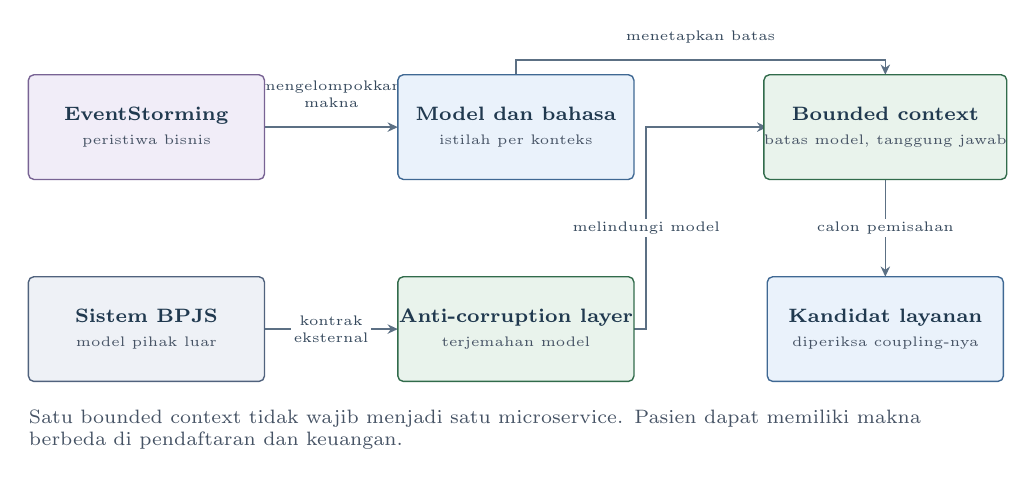
\begin{tikzpicture}[
  x=0.92cm, y=0.95cm,
  kotak konsep/.style={draw, line width=0.5pt, rounded corners=2pt,
    align=center, minimum width=2.999cm,
    minimum height=1.330cm, inner sep=0pt, font=\scriptsize,
    text=konsepJudul},
  peran actor/.style={kotak konsep, fill=konsepIsiActor, draw=konsepGarisActor},
  peran service/.style={kotak konsep, fill=konsepIsiService, draw=konsepGarisService},
  peran control/.style={kotak konsep, fill=konsepIsiControl, draw=konsepGarisControl},
  peran data/.style={kotak konsep, fill=konsepIsiData, draw=konsepGarisData},
  peran outcome/.style={kotak konsep, fill=konsepIsiOutcome, draw=konsepGarisOutcome},
  peran risk/.style={kotak konsep, fill=konsepIsiRisk, draw=konsepGarisRisk},
  panah konsep/.style={-{Stealth[length=1.3mm, width=1.2mm]}, line width=0.6pt,
    draw=konsepPanah},
  panah putus/.style={panah konsep, draw=konsepPanahPutus,
    dash pattern=on 2.5pt off 1.5pt},
  label panah/.style={font=\tiny, align=center, fill=white,
    inner sep=1pt, text=konsepLabel},
  catatan/.style={font=\scriptsize, align=left, anchor=north west,
    inner sep=0pt, text width=12.383cm, text=konsepTeks,
    execute at begin node={\hyphenpenalty=10000\hbadness=10000\relax}},
]
  \definecolor{konsepIsiActor}{HTML}{EEF1F6}
  \definecolor{konsepGarisActor}{HTML}{50627D}
  \definecolor{konsepIsiService}{HTML}{EAF2FB}
  \definecolor{konsepGarisService}{HTML}{3F6893}
  \definecolor{konsepIsiControl}{HTML}{E9F3EC}
  \definecolor{konsepGarisControl}{HTML}{316B4B}
  \definecolor{konsepIsiData}{HTML}{F1EDF8}
  \definecolor{konsepGarisData}{HTML}{786394}
  \definecolor{konsepIsiOutcome}{HTML}{E4F2EC}
  \definecolor{konsepGarisOutcome}{HTML}{236C57}
  \definecolor{konsepIsiRisk}{HTML}{FCEDE7}
  \definecolor{konsepGarisRisk}{HTML}{B36947}
  \definecolor{konsepJudul}{HTML}{20394F}
  \definecolor{konsepTeks}{HTML}{455264}
  \definecolor{konsepLabel}{HTML}{35485C}
  \definecolor{konsepPanah}{HTML}{5C7084}
  \definecolor{konsepPanahPutus}{HTML}{A15D40}
  % Panah dan label lebih dahulu; kotak menutupi sisa latar label.
  \draw[panah konsep] (0.93,0) -- (2.77,0);
  \draw[panah konsep] (4.4,0.7) -- (4.4,0.9) -- (9.5,0.9) -- (9.5,0.7);
  \draw[panah konsep] (9.5,-0.7) -- (9.5,-2);
  \draw[panah konsep] (0.93,-2.7) -- (2.77,-2.7);
  \draw[panah konsep] (6.03,-2.7) -- (6.2,-2.7) -- (6.2,0) -- (7.87,0);
  \node[label panah] at (1.85,0.44) {mengelompokkan\\makna};
  \node[label panah] at (6.95,1.21) {menetapkan batas};
  \node[label panah] at (9.5,-1.35) {calon pemisahan};
  \node[label panah] at (1.85,-2.7) {kontrak\\eksternal};
  \node[label panah] at (6.2,-1.35) {melindungi model};
  \node[peran data] (event) at (-0.7,0)
    {\textbf{EventStorming}\\[0.5pt]{\tiny\color{konsepTeks}peristiwa bisnis}};
  \node[peran service] (bahasa) at (4.4,0)
    {\textbf{Model dan bahasa}\\[0.5pt]{\tiny\color{konsepTeks}istilah per konteks}};
  \node[peran control] (konteks) at (9.5,0)
    {\textbf{Bounded context}\\[0.5pt]{\tiny\color{konsepTeks}batas model, tanggung jawab}};
  \node[peran actor] (bpjs) at (-0.7,-2.7)
    {\textbf{Sistem BPJS}\\[0.5pt]{\tiny\color{konsepTeks}model pihak luar}};
  \node[peran control] (acl) at (4.4,-2.7)
    {\textbf{Anti-corruption layer}\\[0.5pt]{\tiny\color{konsepTeks}terjemahan model}};
  \node[peran service] (layanan) at (9.5,-2.7)
    {\textbf{Kandidat layanan}\\[0.5pt]{\tiny\color{konsepTeks}diperiksa coupling-nya}};
  \node[catatan] at (-2.33,-3.77)
    {Satu bounded context tidak wajib menjadi satu microservice. Pasien dapat memiliki makna berbeda di pendaftaran dan keuangan.};
\end{tikzpicture}
}
\end{frame}

\section{Subdomain dan Ubiquitous Language}

\begin{frame}{\hfill}
  \centering
  \Huge{\textbf{Subdomain dan\\Ubiquitous Language}}
\end{frame}

\begin{frame}{{\Large Tiga Jenis Subdomain}}
  \footnotesize
  \begin{tabularx}{\textwidth}{>{\raggedright\arraybackslash}p{2.6cm}
      >{\raggedright\arraybackslash}X >{\raggedright\arraybackslash}X
      >{\raggedright\arraybackslash}X}
    \hline
    \textbf{Aspek} & \textbf{\textit{Core}} & \textbf{\textit{Supporting}}
      & \textbf{\textit{Generic}} \\
    \hline
    Peran & Pembeda dari pesaing & Khas, bukan pembeda & Sama di semua organisasi \\
    \hline
    Kerumitan & Tinggi, terus dipelajari & Rendah sampai sedang & Tinggi, tetapi
      sudah dipecahkan \\
    \hline
    Bangun atau beli & Bangun dan kuasai sendiri & Bangun sederhana atau beli lalu
      sesuaikan & Beli atau sewa (SaaS) \\
    \hline
    Orang & Tim terbaik & Tim lebih kecil & Pengelola kontrak \\
    \hline
  \end{tabularx}

  \vspace{10pt}
  \small
  Analogi: rendang adalah alasan pelanggan datang ke rumah makan padang; mesin
  kasir cukup dibeli.
\end{frame}

\begin{frame}{{\Large Peta Subdomain Awal Medikara Health}}
  \centering
  \eadiagram{../../figures/ch06-peta-subdomain.tex}
\end{frame}

\begin{frame}{{\Large Kasus Medikara: Nilai Besar Bukan Pembeda}}
  \vspace{10pt}
  \begin{itemize}
    \item Penggajian sekitar 4.800 karyawan: aturan sama untuk semua perusahaan,
          \textit{generic}.
    \item Rekam medis terpadu: sekitar 168.000 dari 1,2 juta kunjungan (14 persen)
          lintas fasilitas, \textit{core}.
    \item Klaim BPJS Kesehatan: misalkan 46 persen pendapatan rumah sakit, tetapi
          aturannya sama untuk semua, \textit{supporting}.
    \item Medikara+ buatan vendor menopang \textit{core}: risiko strategis.
    \item ERP keuangan terpusat tidak perlu diusik.
  \end{itemize}
\end{frame}

\begin{frame}{{\Large Ubiquitous Language}}
  \small
  \begin{itemize}
    \item Kosakata bersama pakar bisnis dan tim teknis, di dalam satu batas model.
    \item Dipakai sama di percakapan, dokumen, diagram, dan kode.
    \item Analogi: gambar kerja bangunan; ``sloof'' dan ``balok'' tidak boleh
          tertukar.
  \end{itemize}
  \footnotesize
  \begin{tabularx}{\textwidth}{>{\raggedright\arraybackslash}p{2.4cm}
      >{\raggedright\arraybackslash}X >{\raggedright\arraybackslash}p{4.6cm}}
    \hline
    \textbf{Istilah} & \textbf{Makna disepakati} & \textbf{Istilah lain ditemukan} \\
    \hline
    Kunjungan & Satu kedatangan ke satu poliklinik pada satu hari & Registrasi,
      episode, \textit{encounter} \\
    \hline
    Pasien baru & Belum punya nomor rekam medis di seluruh jaringan & Baru per
      rumah sakit: sekitar 38.000 nomor ganda \\
    \hline
  \end{tabularx}
\end{frame}

\section{Bounded Context}

\begin{frame}{\hfill}
  \centering
  \Huge{\textbf{Bounded Context}}
\end{frame}

\begin{frame}{{\Large Batas Tempat Satu Model Berlaku}}
  \vspace{10pt}
  \begin{itemize}
    \item \textit{Bounded context}: batas eksplisit tempat satu model dan satu
          bahasa berlaku konsisten.
    \item Di luar batas, istilah yang sama boleh bermakna lain.
    \item Satu model untuk seluruh organisasi besar tidak sepadan biayanya
          (Fowler).
    \item Batas mencakup bahasa, model, data, dan kode.
    \item Analogi: ``kartu'' di bank, di loket rumah sakit, dan di lapangan sepak
          bola.
  \end{itemize}
\end{frame}

\begin{frame}{{\Large Satu Kata, Tiga Makna}}
  \centering
  \eadiagram{../../figures/ch06-makna-pasien.tex}

  \vspace{4pt}
  {\small HL7 FHIR juga memisahkan \textit{resource} Patient dan Coverage.}
\end{frame}

\begin{frame}{{\Large Subdomain dan Bounded Context Sering Tertukar}}
  \footnotesize
  \begin{tabularx}{\textwidth}{>{\raggedright\arraybackslash}p{2.6cm}
      >{\raggedright\arraybackslash}X >{\raggedright\arraybackslash}X}
    \hline
    \textbf{Aspek} & \textbf{\textit{Subdomain}} & \textbf{\textit{Bounded context}} \\
    \hline
    Pertanyaan & Bagian bisnis apa saja yang ada? & Di mana satu model dan satu
      bahasa berlaku? \\
    \hline
    Sifat & Ditemukan dari bisnis (ruang masalah) & Dirancang tim (ruang solusi) \\
    \hline
    Wujud & Peta \textit{subdomain} & Batas model, kode, data, dan tim pemilik \\
    \hline
    Hubungan & Dilayani satu atau beberapa konteks & Idealnya melayani satu
      \textit{subdomain} \\
    \hline
  \end{tabularx}
\end{frame}

\begin{frame}{{\Large Ukuran Bounded Context yang Wajar}}
  \vspace{10pt}
  \begin{itemize}
    \item Terlalu besar: istilah bermakna ganda, banyak tim mengubah model yang
          sama.
    \item Contoh: tabel pasien SIMRS Jakarta berisi 87 kolom, diubah enam modul.
    \item Terlalu kecil: satu perubahan bisnis selalu menyentuh beberapa konteks.
    \item Patokan: satu konteks dimiliki satu tim; satu tim boleh memiliki
          beberapa konteks.
    \item Bila dua kelompok butuh ``kamus'' untuk saling mengerti, di situ ada
          batas.
  \end{itemize}
\end{frame}

\begin{frame}{{\Large Kasus Medikara: Satu Kolom, Tiga Bagian}}
  \vspace{10pt}
  \begin{itemize}
    \item Misalkan Maret 2026: keuangan Depok mewajibkan kolom penjamin sebelum
          pasien dilayani.
    \item Instalasi gawat darurat: sekitar 140 permintaan laboratorium tertahan
          rata-rata 25 menit selama tiga hari.
    \item Laboratorium: label spesimen gagal dicetak untuk pasien rujukan klinik
          mitra.
    \item Aturan itu benar di konteks penagihan, salah di konteks lain.
    \item Seharusnya berlaku sebelum tagihan ditutup, bukan sebelum pasien
          dilayani.
  \end{itemize}
\end{frame}

\section{Context Map}

\begin{frame}{\hfill}
  \centering
  \Huge{\textbf{Context Map dan\\Pola Hubungannya}}
\end{frame}

\begin{frame}{{\Large Hulu, Hilir, dan Analogi Irigasi}}
  \vspace{10pt}
  \begin{itemize}
    \item \textit{Context map}: peta konteks beserta hubungan dan arahnya.
    \item Hulu (\textit{upstream}) memengaruhi hilir (\textit{downstream}), tidak
          sebaliknya.
    \item Petani mengajukan jadwal air: \textit{customer-supplier}.
    \item Petani menyesuaikan jadwal tanam: \textit{conformist}.
    \item Petani membuat kolam penampung: \textit{anticorruption layer}.
  \end{itemize}
\end{frame}

\begin{frame}{{\Large Lima Pola Hubungan}}
  \scriptsize
  \begin{tabularx}{\textwidth}{>{\raggedright\arraybackslash}p{3.1cm}
      >{\raggedright\arraybackslash}X >{\raggedright\arraybackslash}X}
    \hline
    \textbf{Pola} & \textbf{Arti singkat} & \textbf{Biaya atau risiko} \\
    \hline
    \textit{Customer-supplier} & Hilir menyampaikan kebutuhan, hulu merencanakan &
      Butuh forum perencanaan rutin \\
    \hline
    \textit{Conformist} & Hilir memakai model hulu apa adanya & Ikut berubah setiap
      hulu berubah \\
    \hline
    \textit{Anticorruption layer} & Lapisan penerjemah melindungi model hilir & Kode
      dan pemeliharaan tambahan \\
    \hline
    \textit{Shared kernel} & Berbagi sebagian kecil model secara eksplisit &
      Perubahan wajib disepakati dua tim \\
    \hline
    \textit{Open host service} & Protokol terbuka dan terdokumentasi untuk banyak
      pemakai & Hulu memelihara kontrak dan versi \\
    \hline
  \end{tabularx}

  \vspace{8pt}
  \small
  Pola dipilih menurut kenyataan hubungan antartim (hukum Conway), bukan selera
  teknis.
\end{frame}

\begin{frame}{{\Large Context Map Kondisi Saat Ini}}
  \centering
  \eadiagram{../../figures/ch06-context-map.tex}
\end{frame}

\begin{frame}{{\Large Kasus Medikara: BPJS Kesehatan dan SATUSEHAT}}
  \vspace{10pt}
  \begin{itemize}
    \item Klaim di lima SIMRS \textit{conformist}: kode BPJS dipakai langsung di
          layar, tabel, dan laporan.
    \item Misalkan tiga perubahan setahun, rata-rata 30 hari kerja sampai semua
          rumah sakit siap.
    \item Adaptor SATUSEHAT sudah berfungsi sebagai \textit{anticorruption layer},
          tetapi menyimpan aturan klinis.
    \item Usulan: satu \textit{anticorruption layer} di depan konteks klaim.
    \item Biaya tambahan: satu komponen yang dipelihara tim integrasi.
  \end{itemize}
\end{frame}

\section{EventStorming}

\begin{frame}{\hfill}
  \centering
  \Huge{\textbf{EventStorming sebagai\\Lokakarya Kolaboratif}}
\end{frame}

\begin{frame}{{\Large EventStorming}}
  \vspace{10pt}
  \begin{itemize}
    \item Format lokakarya dari Alberto Brandolini untuk mempelajari domain
          bersama.
    \item \textit{Domain event} berbentuk lampau di catatan oranye, diurutkan
          menurut waktu.
    \item Tiga format: Big Picture, Process Modelling, Software Design.
    \item Peserta non-teknis menyumbang sama banyaknya dengan peserta teknis.
    \item Analogi: panitia pernikahan menyusun kronologi hari H bersama.
  \end{itemize}
\end{frame}

\begin{frame}{{\Large Elemen Papan dan Warnanya}}
  \footnotesize
  \begin{tabularx}{\textwidth}{>{\raggedright\arraybackslash}p{2.8cm}
      >{\raggedright\arraybackslash}p{3.0cm} >{\raggedright\arraybackslash}X}
    \hline
    \textbf{Elemen} & \textbf{Warna} & \textbf{Contoh Medikara} \\
    \hline
    \textit{Domain event} & Oranye & Pasien terdaftar \\
    \hline
    \textit{Command} & Biru & Daftarkan pasien \\
    \hline
    Aktor & Kuning, kecil & Petugas loket \\
    \hline
    Sistem eksternal & Merah muda, lebar & Layanan web BPJS Kesehatan \\
    \hline
    \textit{Policy} & Ungu muda & Setiap kali hasil kritis tervalidasi, dokter
      diberi tahu \\
    \hline
    \textit{Hot spot} & Merah muda terang & Siapa menutup kunjungan bila pasien
      pulang sebelum membayar? \\
    \hline
  \end{tabularx}
\end{frame}

\begin{frame}{{\Large Lima Langkah dan Empat Peran}}
  \small
  \begin{enumerate}
    \item Eksplorasi bebas: sekitar 20 menit, tanpa diskusi.
    \item Menegakkan urutan waktu dan menandai \textit{pivotal event}.
    \item Menandai \textit{hot spot}; perdebatan lebih dari dua menit ditinggalkan.
    \item Menambah \textit{command}, aktor, sistem eksternal, \textit{policy}.
    \item Mengelompokkan menjadi kandidat \textit{bounded context}.
  \end{enumerate}
  \vspace{4pt}
  \footnotesize
  Peran: pakar domain, fasilitator, pencatat istilah, penjaga waktu. Daring: dua
  sesi 120 menit, enam sampai sepuluh peserta, warna dikunci.
\end{frame}

\begin{frame}{{\Large Papan Ringkas Alur Rawat Jalan}}
  \centering
  \eadiagram{../../figures/ch06-papan-eventstorming.tex}
\end{frame}

\begin{frame}{{\Large Kasus Medikara: Lokakarya Rumah Sakit Bogor}}
  \vspace{10pt}
  \begin{itemize}
    \item Misalkan dua sesi daring 120 menit, sembilan peserta.
    \item 64 \textit{domain event} dan 11 \textit{hot spot}; tersisa 47
          \textit{event} setelah duplikat dibuang.
    \item Enam kandidat konteks: janji temu, pendaftaran, pelayanan klinis,
          laboratorium, penagihan, klaim.
    \item Misalkan 7 persen berkas klaim dikembalikan, masing-masing dua hari kerja
          perbaikan.
    \item Temuan bahasa: ``diagnosis'' klinis berbeda dari kode diagnosis klaim.
  \end{itemize}
\end{frame}

\section{Kandidat Layanan}

\begin{frame}{\hfill}
  \centering
  \Huge{\textbf{Dari Bounded Context\\ke Kandidat Layanan}}
\end{frame}

\begin{frame}{{\Large Lima Heuristik}}
  \footnotesize
  \begin{tabularx}{\textwidth}{>{\raggedright\arraybackslash}p{3.0cm}
      >{\raggedright\arraybackslash}X >{\raggedright\arraybackslash}X}
    \hline
    \textbf{Heuristik} & \textbf{Pertanyaan pemandu} & \textbf{Contoh Medikara} \\
    \hline
    Kepemilikan data & Siapa satu-satunya pengubah data? & Hasil laboratorium \\
    \hline
    Laju perubahan & Seberapa sering berubah, karena siapa? & Klaim mengikuti BPJS \\
    \hline
    Kebutuhan skala & Apakah bebannya naik turun berbeda? & Janji temu naik 60 persen
      saat vaksinasi \\
    \hline
    Tim pengelola & Tim mana yang menjaganya? & Tim kanal digital \\
    \hline
    Kepatuhan dan risiko & Adakah tuntutan khusus? & Rekam medis elektronik \\
    \hline
  \end{tabularx}

  \vspace{8pt}
  \small
  Team Topologies menyebut batas seperti ini \textit{fracture plane}.
\end{frame}

\begin{frame}{{\Large Konteks Tidak Selalu Sama dengan Layanan}}
  \vspace{10pt}
  \begin{itemize}
    \item Satu konteks menjadi satu layanan: bentuk paling umum.
    \item Satu konteks dipecah karena skala atau risiko berbeda.
    \item Beberapa konteks dalam satu aplikasi: \textit{modular monolith} (Bab 7).
    \item Kesalahan: memecah menurut entitas atau menurut lapisan teknis.
    \item \textit{Capability map} (IT40513) membantu menebak \textit{subdomain}.
  \end{itemize}
\end{frame}

\begin{frame}{{\Large Kasus Medikara: Kandidat Layanan Awal}}
  \scriptsize
  \begin{tabularx}{\textwidth}{>{\raggedright\arraybackslash}p{3.4cm}
      >{\raggedright\arraybackslash}p{2.0cm} >{\raggedright\arraybackslash}X}
    \hline
    \textbf{\textit{Bounded context}} & \textbf{Jenis} & \textbf{Keputusan awal} \\
    \hline
    Janji temu & \textit{Core} & Layanan sendiri \\
    \hline
    Pendaftaran & \textit{Supporting} & Modul dalam aplikasi klinis \\
    \hline
    Pelayanan klinis dan rekam medis & \textit{Core} & Aplikasi klinis, dipecah
      paling akhir \\
    \hline
    Laboratorium & \textit{Supporting} & Layanan sendiri \\
    \hline
    Klaim & \textit{Supporting} & Layanan sendiri dengan \textit{anticorruption
      layer} \\
    \hline
    Akuntansi & \textit{Generic} & Tetap di ERP keuangan \\
    \hline
  \end{tabularx}

  \vspace{6pt}
  \small
  Pencocokan tabel SIMRS Jakarta: hanya 9 dari 14 tabel punya satu konteks
  penulis.
\end{frame}

\section{Aktivitas}

\begin{frame}{{\Large Aktivitas: Lokakarya EventStorming dan Context Map}}
  \small
  \begin{enumerate}
    \item Pilih satu alur layanan pasien; bawa \textit{capability map} dan peta
          dependensi.
    \item Tempel \textit{domain event} berurutan; tandai \textit{pivotal event} dan
          \textit{hot spot}.
    \item Tambahkan \textit{command}, aktor, sistem eksternal; isi glosarium.
    \item Kelompokkan menjadi \textit{bounded context} dengan jenis dan pemilik.
    \item Gambar \textit{context map}, termasuk BPJS Kesehatan dan SATUSEHAT.
  \end{enumerate}
  \vspace{4pt}
  \footnotesize
  Peran: pakar domain dari anggota berlatar kesehatan atau manajemen; anggota
  teknis sebagai fasilitator dan pencatat. Berkas: \berkas{sources/chapter06/}.
\end{frame}

\begin{frame}{{\Large Luaran dan Kriteria Penilaian}}
  \footnotesize
  \begin{tabularx}{\textwidth}{>{\raggedright\arraybackslash}X r
      >{\raggedright\arraybackslash}X}
    \hline
    \textbf{Kriteria} & \textbf{Bobot} & \textbf{Bukti yang dicari} \\
    \hline
    Kelengkapan alur dan \textit{event} & 25 persen & Alur utuh, \textit{hot spot}
      tercatat \\
    \hline
    Kualitas batas \textit{bounded context} & 30 persen & Batas dijelaskan dengan
      \textit{pivotal event}, bahasa, pemilik \\
    \hline
    \textit{Context map} & 25 persen & Semua hubungan punya arah dan pola \\
    \hline
    Glosarium dan kolaborasi & 20 persen & Istilah ganda tercatat \\
    \hline
  \end{tabularx}

  \vspace{10pt}
  \small
  Luaran C2: papan, glosarium, peta \textit{subdomain}, dan \textit{context map}
  kondisi saat ini. Tanpa nama orang dan data pasien di papan.
\end{frame}

\section{Ringkasan dan Latihan}

\begin{frame}{{\Large Ringkasan}}
  \vspace{10pt}
  \begin{itemize}
    \item \textit{Core}, \textit{supporting}, \textit{generic}: menentukan bangun
          atau beli.
    \item \textit{Bounded context}: satu model dan satu bahasa; yang dibagi hanya
          identitas penghubung.
    \item \textit{Context map}: arah hulu-hilir dan pola menurut hubungan antartim.
    \item EventStorming menemukan batas dari alur dan bahasa bisnis.
    \item Batas layanan ditemukan dari bisnis, bukan dari daftar tabel lama.
  \end{itemize}
\end{frame}

\begin{frame}{{\Large Latihan}}
  \small
  \begin{enumerate}
    \item Kata ``pasien'' bisa bermakna berbeda di bagian pendaftaran, keuangan, dan
          laboratorium. Jelaskan cara \textit{bounded context} menangani perbedaan
          makna ini.
    \item Tentukan apakah layanan penagihan di Medikara Health termasuk
          \textit{core}, \textit{supporting}, atau \textit{generic subdomain}.
          Jelaskan konsekuensinya terhadap keputusan membangun sendiri atau membeli.
    \item Mengapa integrasi dengan sistem eksternal seperti BPJS Kesehatan sebaiknya
          dilindungi oleh \textit{anticorruption layer}?
  \end{enumerate}
  \vspace{6pt}
  {\footnotesize Tabel contoh dan lembar isian ada di naskah Bab 6.}
\end{frame}

\end{document}
